\documentclass[../main.tex]{subfiles}
% Preamble
\begin{document}
	\chapter{COMPARATIVA ENTRE ALGORITMOS}
	\newpage
	
	En este cap�tulo, se realiza una comparativa entre los algoritmos implementados (Direct Optimal Basis y CLA) obteniendo los
	resultados con IS Bench.
	
	El siguiente experimento est� basado en conjuntos de implicaciones aleatorias. Se han generado 50 conjuntos combinando dos
	par�metros: el n�mero de implicaciones ( de 5 a 15) y el n�mero de atributos (de 5 a 15). 
	
	Se han desarrollado dos clases para la comparaci�n de los dos algoritmos cuyos detalles se han explicado en el cap�tulo \ref{chap:algoritmosBases} 
	\textit{Algoritmos de c�lculo de bases}. El experimento ha sido ejecutado en un Intel Core i5, 8GB de RAM, con Windows 7 64 bits.
	
	En la Figura \ref{fig:tabla_resumen} se muestran para cada par n�mero de implicaciones atributos, los promedios de los tama�os, cardinalidades y tiempo de ejecuci�n en segundos para ambos algoritmos.
	
	
		\begin{figure}[H]
			\centering
				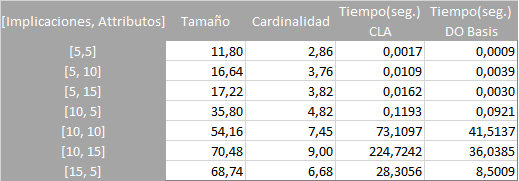
\includegraphics[width=.75\textwidth]{imagenes/tabla_resumen.png}
			\caption{Resultados del experimento}
			\label{fig:tabla_resumen}
		\end{figure}

En la Figura \ref{fig:grafica} se muestra una gr�fica donde se puede apreciar que el tiempo de ejecuci�n del algoritmo CLA aumenta a medida que aumenta la cardinalidad de los resultados. Sin embargo, el algoritmo Direct Optimal Basis tambi�n lo hace pero de una forma m�s moderada.

	\begin{figure}[h]
		\centering
			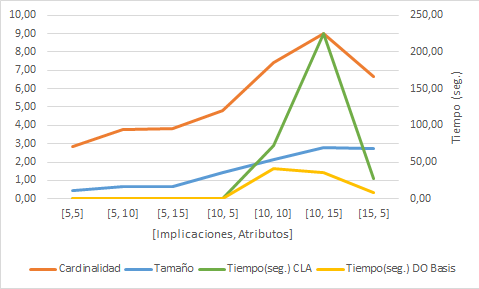
\includegraphics[width=.75\textwidth]{imagenes/grafica.png}
		\caption{Gr�fica de resultados}
		\label{fig:grafica}
	\end{figure}

	
\end{document}



